\section{因子—波动率}
我们提到资产的波动率时,是指价格的标准差,还是收益的标准差。
波动率可以分为实际波动率, 历史波动率, 隐含波动率,预测波动率等。
%先放代码, \href{/Users/nymath/Desktop/Notes/LianHai/code}{123}
\subsection{波动率及其度量}
通常我们的说的波动率,指的是收益率的不确定性,常用标准差进行衡量。
\begin{sdefinition}{波动率的种类}{}
\begin{itemize}
	\item Historical(Realized) Volatility: 
\end{itemize}
\end{sdefinition}

\subsubsection{Realized Volatility}
我们假定收益率服从正态分布。最常用的做法便是利用收盘价计算收益率(简单收益?对数收益?后者),然后计算收益率的年化标准差。
而且,均值为0。
$$
\tcbhighmath{
	\hat \sigma_{cc} = \sqrt{\frac{252}{n}\sum_{i=1}^nr_i^2}
}
$$
虽然简单但没有充分利用市场信息


$$
\tcbhighmath{
	\hat \sigma_{HL} = \sqrt{\frac{1}{4\ln{2}}\frac{252}{n}\sum_{i=1}^n\ln^2{(\frac{H_i}{L_i}})}
}
$$
考虑高开低收
$$
\tcbhighmath{
\hat \sigma_{H L O C}=\sqrt{\frac{252}{n} \sum_{i=1}^n\left[\frac{1}{2} \cdot\left(\ln \frac{H_i}{L_i}\right)^2-(2 \ln 2-1) \cdot\left(\ln \frac{C_i}{O_i}\right)^2\right]}
}
$$
更进一步,我们还可以考虑隔夜的价差(这个专业术语应该怎么说呢?跳空)
$$
\tcbhighmath{
\hat{\sigma}=\sqrt{\frac{252}{n} \sum_{i=1}^n\left[.5\left(H_i^*-L_i^*\right)^2-.39\left(C_i^*-O_i^*\right)^2+\left(O_i^*-C_{i-1}^*\right)^2\right]}
}
$$
如果是日内的话,应该如何估计呢?系数仍然有效吗?
此外上述办法,我们是否可以换成半方差呢?


\subsubsection{Implied Volatility}
我们可以利用Black-Scholes,结合期权的价格,反解波动率。

\subsubsection{Conditional Volatility}
总波动可以利用ARMA-GARCH模型的估计结果,得到条件波动率的估计值,当然也有我们前面提到的特质波动率模型(我们用条件方差的期望度量特质波动率,所以问题就在于这个条件是什么)

\begin{figure}[hbt]
	\centering
	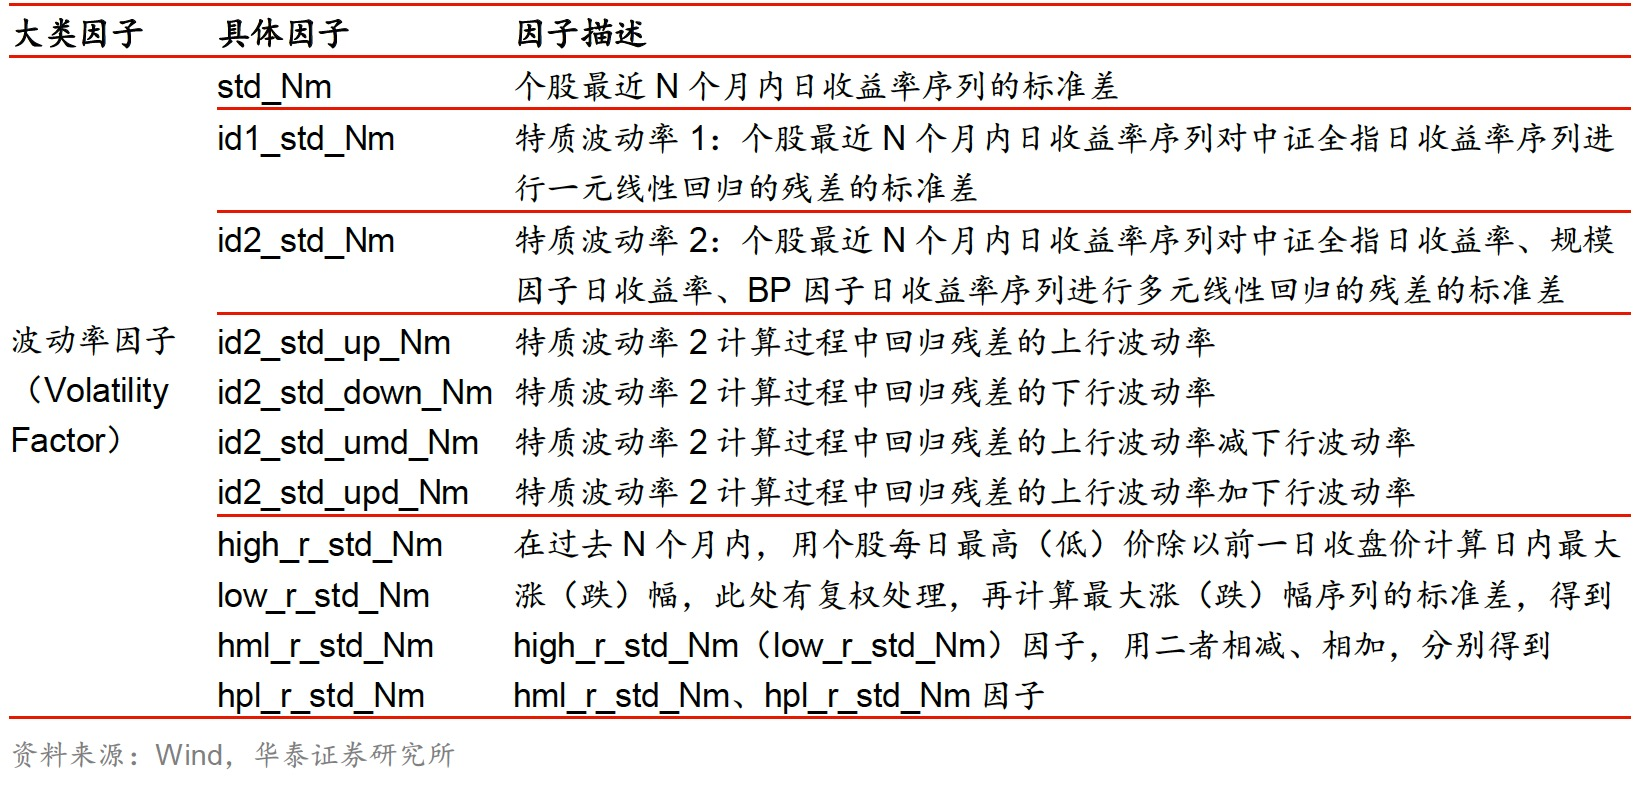
\includegraphics[scale=0.3]{figure/波动率因子_华泰.pic.jpg}
	\caption{波动率因子及其描述}
\end{figure}
	
有一个问题,最大涨幅如何计算,














